\documentclass[12pt]{phage3slides} %

\title[GGA]{Galaxy Genome Annotation: Galaxy and GMOD for Annotation, Teaching, and Genomic Databases}
\author[ER, BG, ND, AB]{Eric Rasche, Bj\"orn Gr\"uning, Nathan Dunn, Anthony Bretaudeau}

\begin{document}
\frame{\titlepage}

% GMOD projects have long provided powerful open-source tools to the
% bioinformatics community, but have historically been hard to configure
% and integrate. The Galaxy Genome Annotation (GGA) group provides a
% highly integrated set of Dockerized GMOD projects allowing for more
% widespread use of these tools in new contexts for system
% administrators wishing to deploy the suite. Our projects include
% maintenance of the Galaxy-Apollo bridge tools, Galaxy-Tripal and Chado
% tooling, and containerized versions of various GMOD projects which are
% configured to easily integrate with the rest of the suite.

% This talk will explore the use of this suite in the context of a real
% life use-case, an undergraduate phage annotation course. We will cover
% the GGA suite as well as various integrations, workflows, training
% materials, and tools that were built and made available in support of
% GGA.

% Very interesting subject. We encourage the presenters to focus on 3-4 key
% aspects of the project rather than try to cover every aspect.

\section{Data Analysis}
\begin{frame}{Data Analysis for Genome Annotation}
	\begin{itemize}
	\end{itemize}
\end{frame}


{%
  \usebackgroundtemplate{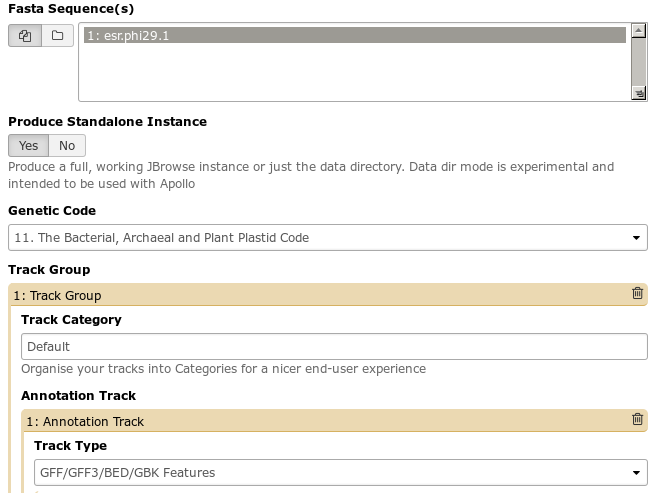
\includegraphics[height=\paperheight,width=\paperwidth]{gx-tool.png}}
  \setbeamertemplate{navigation symbols}{}
  \begin{frame}[plain]
  \end{frame}
}


\section{Q\&A}
\begin{frame}{Q\&A}
    Thank you \\\ \\
    \begin{center}
        \begin{tabular}{rl}
            \color{gray} GGA GitHub       & \href{https://galaxy-genome-annotation.github.io/}{galaxy-genome-annotation.github.io}\\
            %\color{gray} E. Rasche GitHub & \href{https://github.com/erasche}{github.com/@erasche}\\
            %\color{gray} E. Rasche Email  & \href{mailto:hxr@hx42.org}{hxr@hx42.org}\\
            %\color{gray} GPG Fingerprint  & \texttt{F063 D331 6E63 E7B5 23FD}\\
                                          %& \texttt{B9EA C527 B0FC 0AF6 3592}
            \end{tabular}\\[1cm]
            %\logosTamuCPT
            \fundingNSFABIannotation
    \end{center}
\end{frame}

\end{document}
